\chapter{Evaluation}
\label{chap:07_evaluation}
%
\todo{Describe Chapter}

Möglich:
1. Effizienz Auto-Scaler
- Dynamisch skalieren vs statische Anzahl - > was ist schneller

2. GPU Worker
Ab wievielen statischen Worker mit CPU ONLY wird dieselbe Leistung erreicht

\section{Experimental Environment}
The experiments have been conducted on a NVIDIA DGX.
Table AB describes the hardware available on the DGX.
Two of the eight GPUs have been available to conduct the experiments.


The DGX is a live-system as being mentioned in Section XY. Therefore not all available hardware resource have been exclusively available to conduct these experiments.

\section{Experiments}
% Intro
The performance of the computing environment is measured on two widely used machine learning algorithms.
% Explain
In both experiments, a machine learning model is trained on the computing environment using Apache Spark. Furthermore, each benchmark is evaluated using three different configurations:
\begin{enumerate}
\item Using a static number of Apache Spark worker to evaluate the performance of using only CPUs 
\item Using a static number of Apache Spark worker with GPU acceleration enabled
\item Dynamically scaling the number of CPU-only Apache Spark worker nodes using the \textit{Auto-Scaler}
\end{enumerate}
% DIfference between GPU and CPU
The performance difference between GPU accelerated worker nodes and CPU-only worker nodes is explored using two different configurations of the implementation.


% The algorithm
The two benchmarks are:
\begin{itemize}
\item XGBoost classification model using the \textit{Fannie Mae’s Single-Family Historical Loan Performance Dataset}\footnote{Downloaded from: \url{https://docs.rapids.ai/datasets/mortgage-data} (Accessed: 2021-02-06)}\cite{Fannie2021Mortgage}

\item XGBoost regression model using a Taxi fare dataset\footnote{The Taxi dataset is available at: \url{https://github.com/NVIDIA/spark-xgboost-examples/tree/spark-3} (Accessed: 2021-02-06)}
\end{itemize}
% Source
The source code and the dataset used in these experiments are available on Github on the \textit{spark-xgboost-examples}\footnote{spark-xgboost-examples - \url{https://github.com/NVIDIA/spark-xgboost-examples/tree/spark-3} (Accessed: 2021-02-06)} repository from NVIDIA.
% The two diff impl conf
The repository provides a \textit{mortgage} and a \textit{taxi} application. Both applications come with a CPU-only implementation and a GPU implementation.

% supervised
Both classification and regression algorithms are supervised machine learning algorithms.
% whats supervised
The goal of supervised machine learning algorithms is to train a model by finding patterns in labeled data. Then, the model is used to predict labels on new data based on the learned labels.
% Classification
The classification algorithm identifies the category of a label.
% Regression
A regression algorithm predicts a continuous numeric value \cite{Mcdonald2020SparkRapids}.


\subsection{Mortgage Experiment}
% Intro
In this experiment a XGBoost classification model is trained.
% What it tries
The model is trained to 


% Dataset

%The goal of this notebook is to show how to train a XGBoost Model with Spark RAPIDS XGBoost library on GPUs. The dataset used with this notebook is derived from Fannie Mae’s Single-Family Loan Performance Data with all rights reserved by Fannie Mae. This processed dataset is redistributed with permission and consent from Fannie Mae. This notebook uses XGBoost to train 12-month mortgage loan delinquency prediction model .


\subsection{Taxi Experiment}
% Intro
This experiment train a XGBoost regression model to predict a fare amount of a taxi trip based on the amount of passengers and the trip distance.
% The dataset
The dataset used to train the model is provided on the Github repository. FIGURE XY shows the first five lines of the dataset.


\section{Static Worker CPU only}
% Intro
The first experiment is conducted using a static number of Apache Spark worker using only CPUs to evaluate each benchmark.
% Why
The goal of this experiment is, to conduct performance results which can be compared to the GPU accelerated experiment and the Auto-Scaler experiment.
% Specs
Each worker was given a set of resources for each executor: 80 CPU core per executor and 16GB of RAM.
% results
\begin{figure}[h]
\centering
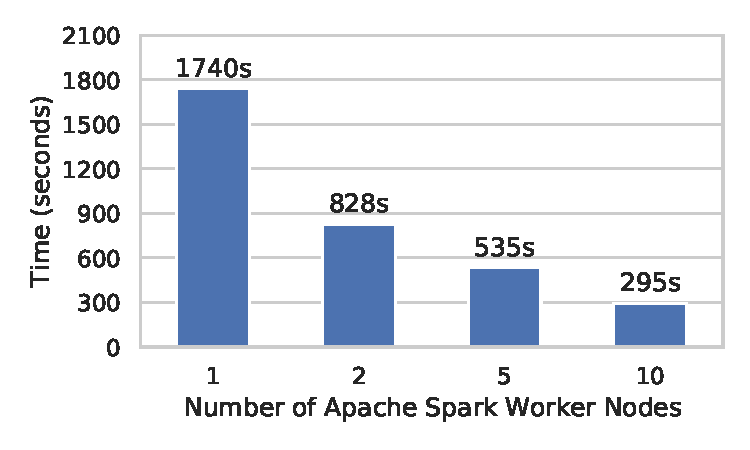
\includegraphics[scale=1]{images/07_evaluation/mortgage/mortgage_cpu_spark-job-mean-time}
\caption{Basic architecture of a GitLab CI/CD pipeline - Source: Authors own model, based on \cite{Gitlab2020Docs}.}
\label{fig:07_mortgage_static-cpu_results}
\end{figure}
%---
\begin{figure}[h]
\centering
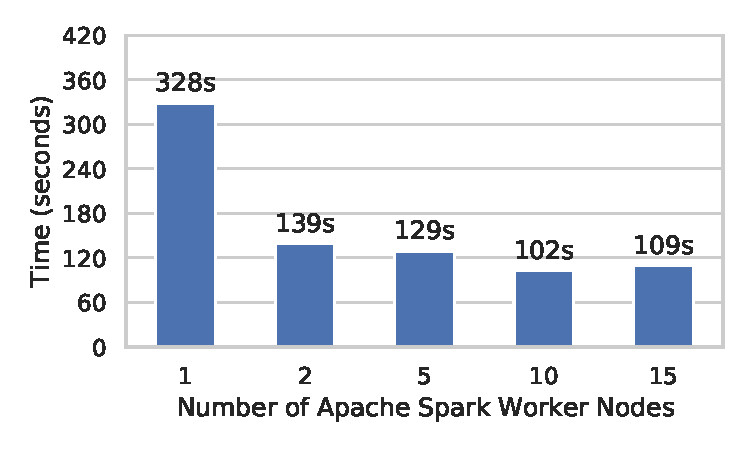
\includegraphics[scale=1]{images/07_evaluation/taxi/taxi_cpu_spark-job-mean-time}
\caption{Basic architecture of a GitLab CI/CD pipeline - Source: Authors own model, based on \cite{Gitlab2020Docs}.}
\label{fig:07_taxi_static-cpu_results}
\end{figure}
% Explain fig
FIG XY illustrates the observed results. It represents the mean execution time in seconds a spark-job needed with the given Apache Spark worker nodes.
% classification
For the classification benchmark, the best result was achieved with 10 worker nodes. Running on 15 worker nodes, the spark job time increased about 6 seconds.
% regression
The regression benchmark achieved the best result with 10 worker nodes as well. Using 15 workers nodes took the spark job time to 109s increased by 7 seconds.
% performance
The performance of all 10 iterations for the classification benchmark is available at ANHANG A and for the regression benchmark at ANHANG B.


\section{GPU Acceleration}
% Intro
The goal of this experiment is to explore the impact of GPU accelerated Apache Spark worker nodes while training machine learning models.
% coars grained
For this experiment, two GPUs have been available. Each benchmark was evaluated 10 times with 1 and 2 GPUs.
%
% vs figure
\begin{figure}[h]
\centering
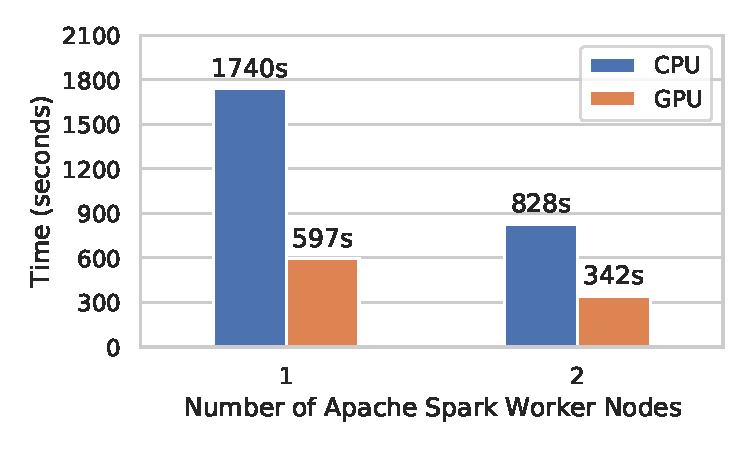
\includegraphics[scale=1]{images/07_evaluation/mortgage/mortgage_gpu_vs_cpu}
\caption{Basic architecture of a GitLab CI/CD pipeline - Source: Authors own model, based on \cite{Gitlab2020Docs}.}
\label{fig:07_mortgage_static-gpu_results}
\end{figure}
%---
\begin{figure}[h]
\centering
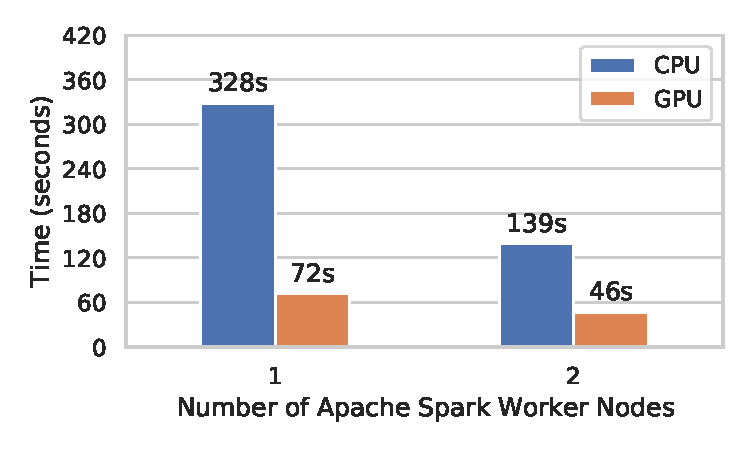
\includegraphics[scale=1]{images/07_evaluation/taxi/taxi_gpu_vs_cpu}
\caption{Basic architecture of a GitLab CI/CD pipeline - Source: Authors own model, based on \cite{Gitlab2020Docs}.}
\label{fig:07_taxi_static-gpu_results}
\end{figure}
% Explain results
The results illustrate the mean time of the spark-job execution time in seconds.
% classification
For the classification algorithm, using 1 GPU accelerated worker was able to decrease the execution time by 1143 seconds, using 2 GPUs a betternes of 486 seconds. Using 1 GPU thats an 2.9x increase and for 2 GPUs an increase of 2.4x.
% regression


\section{Auto-Scaler}
lieber Beide algos in einem diagramm und dann auf die verschiedenen einstellungen in einer tabelle eingehen.

% Intro
To test the impact of the Auto-Scaler while training machine learning applications, both benchmarks have been tested with different configurations. \Tab{table:07_auto-scaler_config_parameter} shows the Auto-Scaler configuration parameters for each benchmark.
% Wheres it from
The configuration parameters are have been choosen in accordance to the results of the static worker experiment.
% Max worker
Both benchmarks in the static worker experiment achieved the best overall performance using 10 worker nodes. Therefore, this value is chosen as the maximum number of worker nodes.
% recurrence
The recurrence factor for the regression experiment was set to 1, because an iteration using 2 worker nodes took 80 SECONDS in mean. Using a higher recurrence factor for this experiment lead to no scaling actions. The target CPU utilization is the mean utilization of each benchmark using 2 worker nodes.
% CPU utilization
The CPU utilization values have been chosen in accordance to the minimum and maximum values of the static worker experiment.
% The configurations
\begin{table}[]
\centering
\begin{tabular}{@{}l|ll@{}}
\toprule
Parameter               & Classification & Regression \\ \midrule
Interval                & 5 seconds      & 5 seconds  \\
Recurrence factor       & 3              & 1          \\
Cooldown period         & 60 seconds     & 60 seconds \\
Target CPU utilization  & 20\%           & 5\%        \\
Minimum CPU utilization & 10\%           & 2\%       \\
Maximum CPU utilization & 25\%           & 10\%       \\
Minimum worker nodes    & 2              & 10         \\
Maximum worker nodes    & 2              & 10         \\ \bottomrule
\end{tabular}
\caption{Auto-Scaler configuration parameter}
\label{table:07_auto-scaler_config_parameter}
\end{table}


% Figure
\begin{figure}[h]
\centering
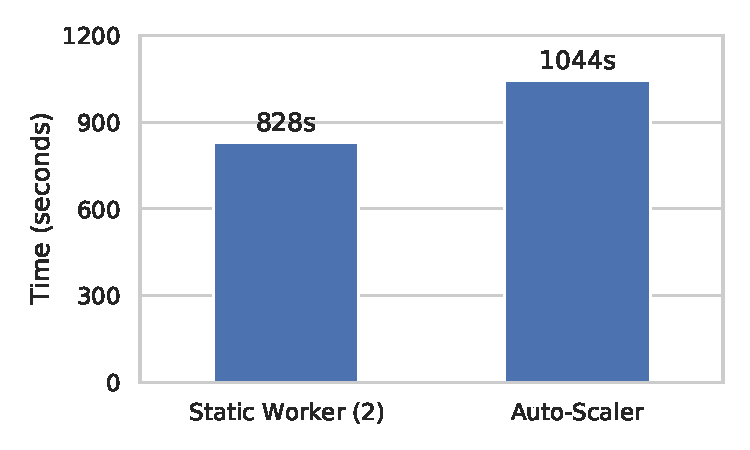
\includegraphics[scale=1]{images/07_evaluation/mortgage/mortgage_auto_scaler_2_worker}
\caption{Basic architecture of a GitLab CI/CD pipeline - Source: Authors own model, based on \cite{Gitlab2020Docs}.}
\label{fig:07_mortgage_auto-scaler_results}
\end{figure}
%---
\begin{figure}[h]
\centering
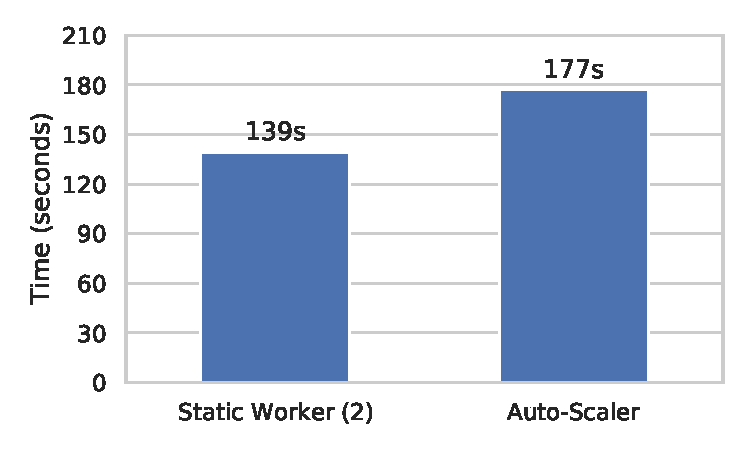
\includegraphics[scale=1]{images/07_evaluation/taxi/taxi_auto_scaler_2_worker}
\caption{Basic architecture of a GitLab CI/CD pipeline - Source: Authors own model, based on \cite{Gitlab2020Docs}.}
\label{fig:07_taxi_auto-scaler_results}
\end{figure}
% Explain
The results, illustrated in FIG A, showed that scaling the number of Apache Spark worker nodes during the training of a machine learning model increased the overall time of the spark-jobs.
% Classification
In the classification benchmark, the Auto-Scaler caused an increase of 216 seconds in comparison of no auto-scaling.
% Regression
Dynamically scaling worker nodes during the regresssion benchmark increased the mean time by 38 seconds.
% Meaning
Given this result, 
